\documentclass[journal]{./IEEE/IEEEtran}
\usepackage{cite,graphicx,amsmath,mathtools,caption,fixltx2e}

\newcommand{\SPTITLE}{Sign Language Translation using Convolutional Neural Networks}
\newcommand{\ADVISEE}{Carlos Miguel E. Canonizado}
\newcommand{\ADVISER}{Jaime M. Samaniego}

\newcommand{\BSCS}{Bachelor of Science in Computer Science}
\newcommand{\ICS}{Institute of Computer Science}
\newcommand{\UPLB}{University of the Philippines Los Ba\~{n}os}
\newcommand{\REMARK}{\thanks{Presented to the Faculty of the \ICS, \UPLB\
                             in partial fulfillment of the requirements
                             for the Degree of \BSCS}}
        
\markboth{CMSC 190 Special Problem, \ICS}{}
\title{\SPTITLE}
\author{\ADVISEE~and~\ADVISER%
\REMARK
}
%\pubid{\copyright~2006~ICS \UPLB}

%%%%%%%%%%%%%%%%%%%%%%%%%%%%%%%%%%%%%%%%%%%%%%%%%%%%%%%%%%%%%%%%%%%%%%%%%%

\begin{document}

% TITLE
\maketitle

% ABSTRACT
% \begin{abstract}
% No abstract yet
% \end{abstract}

% INDEX TERMS
\begin{keywords}
sign language, hand gesture recognition, neural network, convolution, convolutional neural network
\end{keywords}

% INTRODUCTION
\section{Introduction}
Sign language is a system of communication that has been around for years. Its primary usage is to enable communication between deaf and hearing people. The World Health Organization (WHO) \cite{WHO2018} estimated that by 2050, more than 900 million people will have disabling hearing loss. Given this large estimation, it is problematic that only a small percentage of people actually know how to use sign language. One of the most widely used sign languages is the American Sign Language (ASL). The ASL gained its popularity after William Stokoe, Dorothy Casterline, and Carl Croneberg published their Dictionary of American Sign Language on Linguistic Principles in 1965 \cite{Wilcox1991}.
\newline
\indent When it comes to motion gesture technology, the earliest implementation was made possible through the use of gloves with sensors. Depending on the hand movement, signals were decoded by a computer by mapping a combination of signals to unique gestures \cite{Sharma2015}.  Today, technological advancements allow programmers to develop tools that deal with the likes of motion gesture recognition, without the use of any external equipment, aside from cameras. Specifically, Open Source Computer Vision (OpenCV) is one of those tools that provide a set of functionalities to be integrated with programming languages such as Python, allowing real-time manipulation of what a computer sees.
\newline
\indent Another technological advancement which will make this study feasible is the existence of Artificial Intelligence (AI). AI is a broad topic and one of its use many uses is the implementation of neural networks. A neural network is a set of connected processors or neurons which can be activated to produce a desired idea or result \cite{Schmidhuber2015}. Neural networks have different types but for image-related tasks, a convolutional neural network (CNN) is widely used due to its advantages for image classification or categorization \cite{Wu2016}.
\newline
\indent This study aims to develop a mobile application to translate sign language using image or video processing through the implementation of convolutional neural networks in order to fulfill the following:

\begin{enumerate}
\item allow not only sign language to text but also vice-versa;
\item detect and interpret hand gestures regardless of the hand's orientation, color, or size; and
\item interpret dynamic or moving sign language.
\end{enumerate}

\indent Being able to translate sign language to text or vice-versa will be beneficial not only for the deaf community but also for those who are aspiring to learn sign language. Moreover, the communication barrier between the deaf and non-deaf community will be minimized since they will have accessible translators.
\newline
\indent Given that sign language has many variations, it would be difficult to consider these variations all at once because of the existence of overlapping meanings among gestures. Thus, ASL will be used as the standard vocabulary of this study to prevent ambiguities that may arise during implementation.
\newline
\indent The application will cater to mobile users since there are not many viable real-time sign language translators for public use. Since the processors of modern phones are not as powerful as actual computers, the application that will be developed from this study will require internet connectivity to connect to a server that will translate the sign language and train the CNN as more gestures get added to the network.

% RELATED LITERATURE
\section{Related Literature}
For several decades, understanding the deaf community has become a major challenge. Sign language, despite its many variations, is one of the most effective methods that allow the better communication between the deaf and the non-deaf community. Several studies have been conducted to further allow translation of sign language without actually learning the language. One of the most popular is the use of digital image processing as a prerequisite in translation methods such as support vector machines and neural networks.

\subsection{Digital Image Processing}
An image is defined as a two-dimensional function, f(x,y), where x and y are the plane coordinates and the amplitude of f at any coordinate (x,y) is called the intensity of the image at that point \cite{Gonzalez2002}. The intensity of the points would usually have three values representing the Red Green Blue (RGB) color model. Another dimension can be added to RGB which is called RGBa where a is the alpha value that dictates the opacity of the point. These points are called pixels and given that images contain a set of pixels, these pixels can then be interpreted through the use of digital image processing.
\newline
\indent As for digital image processing, it refers to processing digital images by means of a digital computer. This process is done for many reasons, one of which is to enhance the image quality for human interpretation and another is to improve autonomous machine perception \cite{AbriolSantos12018}.
\newline
\indent One common method used in digital image processing is converting a colored image to grayscale. This method will remove the different colors of an image, rendering it to have shades of gray only. Grayscale conversion is usually done during pre-processing and it is achieved by changing every pixel value of an image with the mean of the current pixel's RGB values.
\newline
\indent The ability to turn an image to grayscale will make it easier to interpret the image's values due to the limited amount of color. However, some processes require taking it a step further by converting an image to binary. This means that for every pixel of the image, it would only be either one or zero. Converting an image to binary is done with the use of thresholds.
\newline
\indent Lastly, another important method done in image processing that is also relevant to this study is edge detection. Edges are the boundaries between the regions of an image; edges could also be referred to as the outline of the objects in an image \cite{Sharma2013}. Edge detection is useful because it reduces the amount of data and it filters out useless information, at the same time, preserves the important structural properties of an image.

\subsection{Previous Studies on Sign Language Translation}
Throughout the years, a lot of implementations regarding sign language translation have been developed.
\newline
\indent One implementation is done with the help of a Support Vector Machine (SVM). An SVM is used for analyzing data through classification, regression, and outliers detection. Additionally an SVM is a supervised machine learning algorithm that is reliant on plotted data points. Villamor \cite{Villamor2018} was able to utilize an SVM in sign language translation through the following process: first, given an input image, the background and hand are identified. After that, the features of the hand are detected, examples of these features are the center of the palm, finger defect points, and finger vectors. These data are then plotted in an n-dimensional space, where n is the number of features. Once the points are plotted, the image is classified by finding the difference of two sets of points. The classification may be in a form of labels or definitions and in this case, Villamor classified a hand gesture according to its definition.
\newline
\indent Another method that was used in translating sign language is color segmentation and neural networks. For this method, Akmeliawati \cite{Akmeliawati2007} used custom-made gloves to gather necessary data from the signer. Since there is a lot of unwanted data captured in an image or video, the frames were segmented according to the color that was visible in the gloves. This makes the translation easier since the program expects certain colors for each feature like yellow for the palm, purple for the thumb, red for the index and ring finger, and blue for the middle and pinky finger.
\newline
\indent The fingers produce data which are called vectors. A vector is a collection of numbers and for each finger, there is one xyvector giving a total of five xyvectors per hand. The weights of the data from these vectors are then fed into a neural network, to be specific, an artificial neural network (ANN). The ANN that Akmeliawati used had three neural networks: one for recognizing the alphabet, another for numbers, and the third one for word signs. After traversing these layers, a value will be returned if ever the ANN correctly classifies the input gesture. The use of color segmentation and ANN allowed Akmeliawati to detect dynamic signs such as fingerspelling. However, the slight disadvantage this has with the SVM is that external equipment is needed.

\subsection{Neural Network}
Based on basic neurobiology, a human brain consists of billions of nerve cells or neurons. These neurons communicate through electrical signals in the voltage of the cell wall or membrane. Essentially, each neuron receives thousands of connections from other neurons resulting to a multitude of incoming signals which reach the cell body \cite{Gurney1997}. Therefore, a connection of neurons can be called a neural network. In computer science terms, a neural network is called as is but it can also be referred to as an artificial neural network (ANN).
\newline
\indent An artificial neural network contains a set of processing units or nodes which simulate neurons and are interconnected by a set of weights. These weights are numerical and are passed onto the nodes. The nodes are simple computing elements that would mimic the behavior of neurons by comparing the current weight with a threshold. This process is called the activation function where if the threshold of the current node is exceeded by the input weight, the node activates and it can pass the weight to other connected nodes until it reaches a certain output \cite{Cross1995}.
\newline
\indent As opposed to real neural networks, artificial neural networks have a predefined structure. An artificial neural network has an input layer, an output layer, and hidden layers in between. The number of neurons in the input layer is dependent on the number of features in a given data set. After an input is sent to the input layer, it is then fed into the hidden layers. There can be any amount of hidden layers depending on the network model and data size. Each hidden layer can also vary in the number of neurons or nodes but generally, the nodes are greater than the number of features. The result from each layer is computed by getting the product from the matrix multiplication of the previous layer's output with the learnable weights of the current layer and by adding learnable biases, followed by the activation function. Finally, the output from the hidden layers is fed into a logistic function such as a sigmoid which converts the output of each class into the probability score of each class \cite{MishraND}. The equation for a sigmoid function is given by:
\newline
\begin{equation}
\sigma(x) = \frac{1}{1+e^{-x}}
\end{equation}
\newline
\indent Errors are inevitable when transitioning from one layer to another which is why there are methods that attempt to minimize them. One common error reduction method is backpropagation. Backpropagation is done by comparing the output of the network with the true output while propagating the error back through the network, altering the weights and biases of the connections between the network elements to make the network's response more accurate next time \cite{Cross1995}.

\subsection{Convolution}
In digital image processing, the characteristics of an image are often modified. The modification is done through convolution and the output can be a smoothened, sharpened, intensified, or enhanced image. In addition, the process of convolution can result to the edges of an image. Therefore, a convolution can be defined as a general purpose filter effect for images \cite{Ludwig2007}. To be able to apply convolution, kernels are used. A kernel is a matrix of numbers which is of the size N x N where N is an odd number. An example of a kernel is given by:
\newline
\begin{equation}
\begin{bmatrix}
1&2&1\\ 
2&4&2\\ 
1&2&1 
\end{bmatrix}
\end{equation}
\newline
\indent The convolution formula is defined by the equation:
\newline
\begin{equation}
O(x,y) = \left | \frac{\sum_{i=-(n-1)/2}^{(n-1)/2} \sum_{j=-(n-1)/2}^{(n-1)/2}f\textsubscript{ij}d\textsubscript{ij}}{F} \right |
\end{equation}
\newline
\indent In the formula above, O(x,y) is the output pixel, x y of image O; n is the size of the convolution kernel; f\textsubscript{ij} is the value of the kernel at i,j; d\textsubscript{ij} is the value at pixel i,j; and F is the sum of values of the kernel \cite{AbriolSantos22018}.

\subsection{Convolutional Neural Network}
Convolutional neural networks (CNNs) are similar to traditional neural networks in a sense that they are comprised of neurons that are optimized through learning. Each node or neuron will still receive an input and perform activation functions. The main difference is that CNNs are primarily used for pattern recognition with images \cite{OShea2015}.
\newline
\indent O'Shea \cite{OShea2015} states that one of the largest limitations of regular neural networks is the lack of computational power required to compute data from images. Handwritten digits can be viable in regular neural networks since the image dimensions could be as small as 28 x 28. However, if we take a larger colored image input of 64 x 64, then the number of neurons for the first layer increases to an overwhelmingly large number of 12,288.
\newline 
\indent With traditional neural networks, there is a minimum of three layers: the input, output, and hidden layers in between. In CNN, there are additional layers namely: convolutional layer, pooling layer, and fully-connected layers. The process of recognizing an image in CNN is done by passing an input image to the input layer. The input layer will hold the pixel values of the image. Next, the convolutional layer will compute for the output of the neurons. The output is then passed to the pooling layer which will reduce the number of activation parameters by downsampling through a rectified linear unit (ReLu). After that, the fully-connected layers will attempt to produce a probability classification of each class, similar to that of an artificial neural network. Note that convolution and pooling may be done several times to arrive at higher level features of the image.

% MATERIALS AND METHODS
\section{Methodology}
This study will focus on translating different hand gestures to their respective definitions in ASL. An Android application will serve as the user interface and in order to correctly classify the hand gestures, a computer program will be implemented using Python along with other utilities. The whole translation process will be done in a separate Python server to minimize the heavy processes done on the mobile phone.

\subsection{System Requirements}
The following will be used to develop and implement the mobile application:

\begin{itemize}
    \item A smartphone running on Android version 5.1.1 or higher for the user interface;
    \item Android Studio version 3.2.1 or higher for creating the mobile application;
    \item Windows or Linux operating system to run the Python server;
    \item Python version 3.6 or higher and Python Flask 1.0 or higher for creating the server;
    \item OpenCV version 3.4.2 or higher for digital image processing; and
    \item TensorFlow version 1.0 or higher for CNN development.
\end{itemize}

\subsection{Data Gathering}
The data that will be used in this study will be sign language gestures that are available from different sources such as Google's Dataset Toolbox and Kaggle, a site where a community of data scientists freely share their data and machine learning information. In addition, the researcher will also take his own pictures for the accumulation of more hand gestures. The amount of training data to be used is around 500 images per gesture but more than that is better.

\subsection{Mobile Application}
The mobile application will be named ``Sign Me Up!'' which will have three functionalities: one for translating sign language to text, another for translating text to sign language, and lastly, one for adding a new gesture. It will be made available for Android using Android Studio as the integrated development environment (IDE). The wireframe can be seen in the appendix.

\subsection{Translation}
The process of translating text to sign language will just be dependent on the gestures available. A sequence of images will be shown per letter or phrase that needs to be translated. However, the process of translating sign language to text can be found in Figure 1. Note that all the steps in translating sign language to text will be implemented using Python as the programming language, OpenCV for digital image processing, and Tensorflow for CNN development.
\newline
\newline
\newline
\newline
\newline

\begin{figure}[ht!]
    \centering
    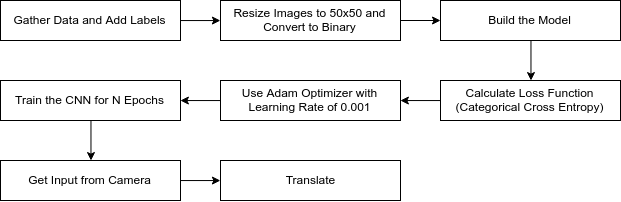
\includegraphics[width=1\linewidth]{./images/methodology.png}
    \caption{Sign Language to Text Translation}
    \label{fig:label1}
\end{figure}

\subsubsection{Labeling the Data}
Once enough data has been gathered, all the images per gesture will be stored in an individual folder and labels will be manually added depending on the definition of the gestures in ASL.
\newline
\subsubsection{Image Processing}
Before using the available data, each image must first be processed using OpenCV. All images will be resized to 50x50 pixels using OpenCV's resize function. After that, the images will be converted to grayscale and then to binary using adaptive thresholding. Other preprocessing methods such as sharpening or enhancing images will be used if deemed necessary.
\newline
\subsubsection{Building the Model}
After processing the images, the model can now be created. The input layer will hold all the pixel values of the image. The hidden layers will contain N convolution and pooling layers before being stacked into a fully-connected layer. The output of probabilities will be dependent on the gestures that were defined in the labeled data. For this CNN model, the activation function to be used is a Rectified Linear Unit (ReLu) which is given by:

\begin{equation}
R(x) = max(0,x)
\end{equation}
\indent The ReLu removes all negative values from the filtered images and replaces it with zeros in order to prevent the values from summing up to zero.
\newline
\indent Once the model is supplied with the appropriate parameters such as the number of filters and stride size for the convolution and the window size for the pooling layer, the loss can be calculated using categorical cross entropy.
\newline
\subsubsection{Categorical Cross Entropy}
It is important to minimize any loss in the CNN and one way to do that is to tune the parameters during training. To be able to calculate for the loss or degree of error, a categorical cross entropy function will be used. Its formula is given by:
\begin{equation}
-\frac{1}{N}\sum_{i=1}^{N}\sum_{c=1}^{C}1y_{i}\epsilon C_{c} logp_{model}[y_{i} \epsilon C_{c}]
\end{equation}
\indent In the formula above, the double summation is over the number of observations i whose number is N and the categories c whose number is C. The term 1y\textsubscript{i} is the indicator of the ith observation belonging to the cth category. This function returns a vector of C probabilities.
\newline
\subsubsection{Adam Optimizer}
The Adam Optimizer is the most complex part of the CNN and is the default go-to optimizer. It is used to update the weights of the network in order to arrive at better results. This optimization method is already available for ease of use in the Tensorflow API. Ideally, a slower learning rate is preferred since a smaller step size would lead to better approximations.
\newline
\subsubsection{Training}
Lastly, the epochs refer to the number of iterations that the CNN will train for. Once the network is done training, translation can be done by using the detected hand gestures from the camera as input.
\newline
\subsubsection{Getting Input}
The smartphone's camera will serve as the source of input for translation. But before being able to extract any data from it, the hand must be detected first. Hand detection will be done by applying background subtraction to the current frame and converting the result to binary. Since there will be a lot of unnecessary elements, the biggest contour must be found which will most likely be the hand. After the contour of the hand is found, it will be the only one filled. This will give us a result of a binary image of the input hand which will be passed into the CNN for translation. A sample input can be seen in the initial results.

% INITIAL RESULTS FOR SP 1
\section{Initial Results}
After testing with a laptop's camera, the background can now be subtracted and the program can easily detect a hand. This is assuming that only one hand at a time is being detected and the color of the hand is not similar to the background.

\begin{figure}[ht!]
    \centering
    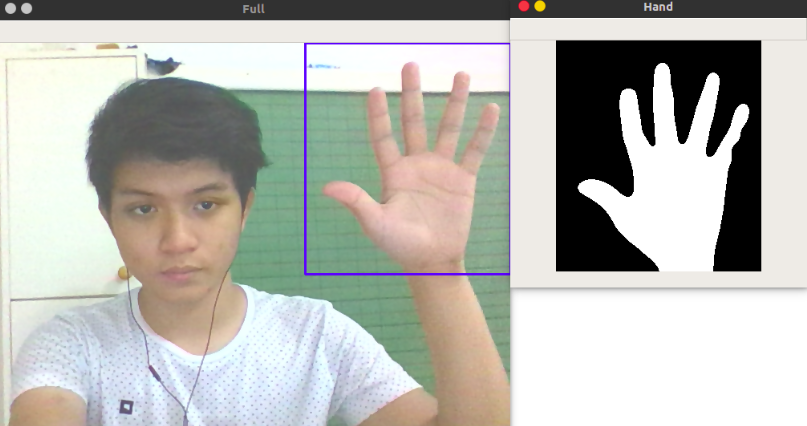
\includegraphics[width=.8\linewidth]{./images/init1.png}
    \caption{Hand detection 1}
    \label{fig:label1}
\end{figure}

\begin{figure}[ht!]
    \centering
    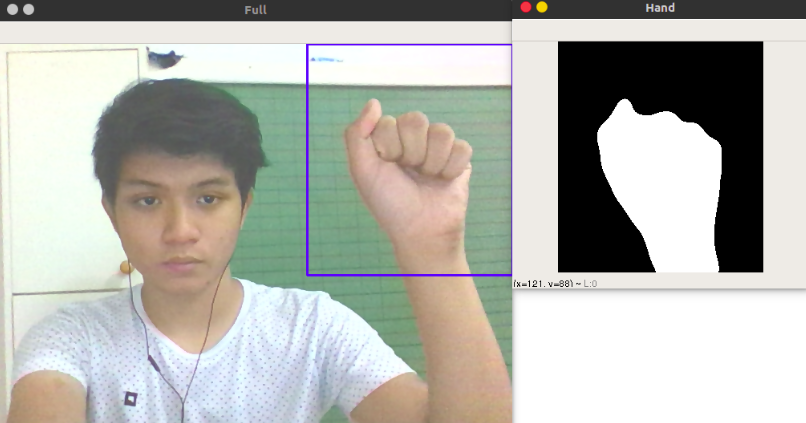
\includegraphics[width=.8\linewidth]{./images/init2.png}
    \caption{Hand detection 2}
    \label{fig:label1}
\end{figure}

% RESULTS AND DISCUSSION
% \section{Results and Discussion}
% No results yet

% CONCLUSION AND FUTURE WORK
% \section{Conclusion and Future Work}
% No conclusion yet

% BIBLIOGRAPHY
\bibliographystyle{./IEEE/IEEEtran}
\bibliography{./cs190}

% APPENDIX
\appendix
\begin{figure}[ht!]
    \centering
    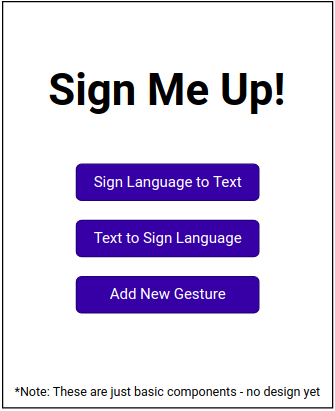
\includegraphics[width=.95\linewidth]{./images/1.png}
    \caption{Menu screen}
    \label{fig:label1}
\end{figure}

\begin{figure}[ht!]
    \centering
    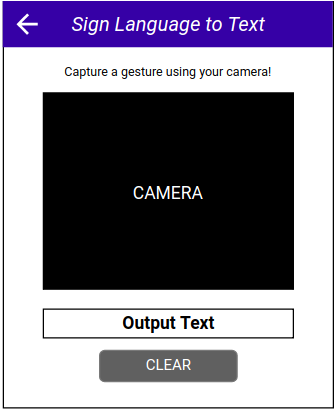
\includegraphics[width=.95\linewidth]{./images/2.png}
    \caption{First functionality}
    \label{fig:label2}
\end{figure}

\begin{figure}[ht!]
    \centering
    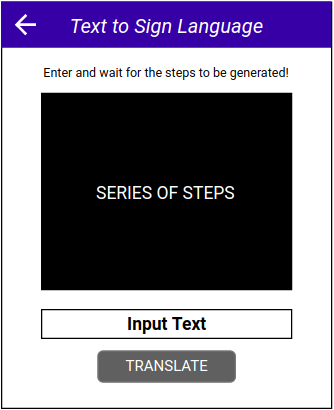
\includegraphics[width=.95\linewidth]{./images/3.png}
    \caption{Second functionality}
    \label{fig:label3}
\end{figure}

\begin{figure}[ht!]
    \centering
    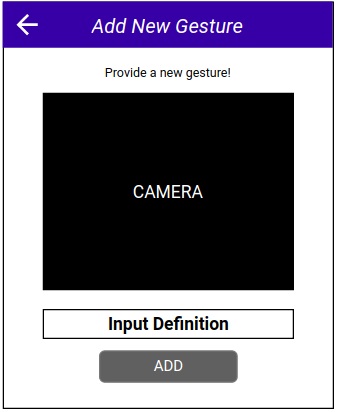
\includegraphics[width=.95\linewidth]{./images/4.png}
    \caption{Third functionality}
    \label{fig:label4}
\end{figure}

\end{document}
 
